\scanpage{40}
% archive sheet number: 39
\[
0\longrightarrow K^*\longrightarrow\prod_{\mathrm{local}}K_x^*\longrightarrow{\unsure{\mathbb{J}|\mathscr{J}}}_C(\bar{k})\longrightarrow0
\]
% margin note slanted, circled
\margin{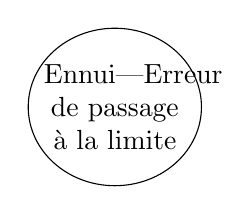
\begin{tikzpicture}\node[text width=1.8cm,align=center] (n) {\uline{{\unsure{Ennui|Erreur}} de passage à la limite}};\draw (n.center) ellipse (1.1cm and 1cm);\end{tikzpicture}}
\margin{\textcircled{?}}
\[
\begin{aligned}
\widehat H^*(\Gamma,K^*)&=0&&\text{par le théorème de Tsen global}\\
\widehat H^*(\Gamma,K_x^*)&=0&&\text{''}\qquad\text{local}
\end{aligned}
\]
d'où
\[
\widehat H^*(\Gamma,\mathbb{J}_C(\bar{k}))=0\qquad\text{géométrique}
\]
\[-\]
En particulier

\deleted{${\unsure{H}}\ C^*(\Gamma,\mathbb{J}_C({\unsure{k|\bar{k}}}))$ est une \uline{résolution} de ${\unsure{\mathbb{J}}}$. \inserted{$H^0(C^*(\Gamma,\mathbb{J}_C({\unsure{\bar{k}}})))$}}

$C^*(\Gamma,\mathbb{J}_C(\bar{k}))$ est une \uline{résolution} de $H^0(\Gamma,\mathbb{J}_C(\bar{k}))$

Or on a, en vertu de $H^1(\Gamma,K^*)=0$
\[
\begin{aligned}
H^0(\Gamma,\mathbb{J}_C(\bar{k}))&=H^0\left(\prod_{\substack{\mathrm{local}\\x\in X}}K_x^*\right)/\operatorname{Im}H^0(K^*)\\
&=\left(\prod_{\substack{\mathrm{local}\\x'\in X'}}K_{x'}^{\prime *}\right)/K^{\prime *}=\mathbb{J}_{C'}(\bar{k})
\end{aligned}
\]
C'est là une résolution \inserted{(Mais qui {\unsure{ne sont pas|ne soit pas|n'est pas}} ``{\unsure{admissibles|admissible}}'')} de \uline{$\pi$-groupes}

D'où
\[
H^*(\pi,\mathbb{J}_{C'}(\bar{k}))\Longleftarrow H^p\left(H^q\left(\pi,\underbrace{C^*\left(\Gamma,\mathbb{J}_C(\bar{k})\right)}_{C^*(\Gamma,\mathbb{J}_C)(\bar{k})}\right)\right)
\]
\[
\begin{aligned}
q>0\qquad H^q(\pi,C^*(\Gamma,\mathbb{J}_C)(\bar{k}))
&=\deleted{{\unsure{C^*}}}H^q(\pi,C^*(\Gamma,\mathbb{Z}))=0\\[-2pt]
&\qquad\text{(Lang)}
\end{aligned}
\]
\margin{trivial car $C^*(\Gamma,\mathbb{Z})$ est $\simeq\mathbb{Z}^{{\unsure{(I)|I}}}$ \deleted{{\unsure{\mathbb{Z}}}}}
\[
q=0\qquad C^*(\Gamma,\mathbb{J}_C(\bar{k}))^\pi=C^*(\Gamma,\mathbb{J}_C(k))
\]
\figure{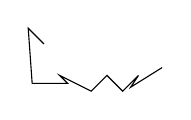
\begin{tikzpicture}\draw (0,.5)--(-.2,.7)--(-.15,0)--(.3,0)--(.2,.1)--(.6,-.1)--(.8,.1)--(1,-.1)--(1.2,.1)--(1.1,-.05)--(1.5,.2);\end{tikzpicture}}
